\documentclass[11pt]{amsbook}

\usepackage{../HBSuerDemir}	% ------------------------
\usepackage{multicol}
\usepackage{fancyhdr} % Header/Footer
\pagestyle{fancy}
\thispagestyle{fancy}
\fancyfoot{}
\fancyfoot[L]{\footnotesize 
	Freshman Calculus by Suer \& Demir  \textbf{DRAFT} \\
	\LaTeX ~by Haluk Bingol 
	\href{http://www.cmpe.boun.edu.tr/~bingol}
	{http://www.cmpe.boun.edu.tr/bingol} 
	%\large 
	%\footnotesize 
	\today}
\fancyfoot[R]{{\thepage} of \pageref{LastPage}}

\begin{document}
	
	% ++++++++++++++++++++++++++++++++++++++
	\hPage{b2p2/278}
	% ++++++++++++++++++++++++++++++++++++++
	
	\centerline{\thepage}
	\bigskip
	
	\begin{enumerate}
	\noindent
	\begin{minipage}{0.6\textwidth}\raggedright
		\item[]
		\begin{enumerate}
			\item[b)]\quad $D = {(x, y): |x^2 - y^2| \neq 0, xy>0}$
		\end{enumerate}
	\end{minipage}
	\hfill%
	\begin{minipage}{0.3\textwidth}
		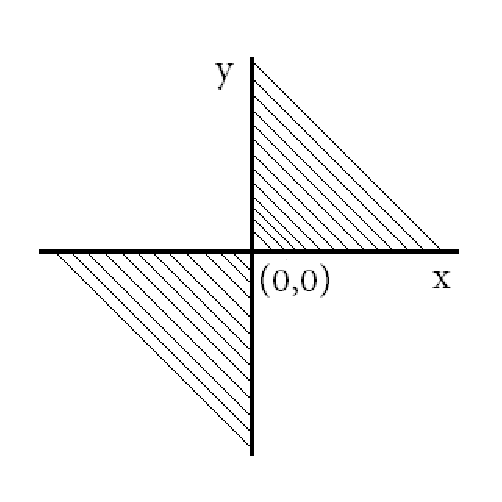
\includegraphics[width=0.8\linewidth]{images/b2p2-278-2b.eps}
	\end{minipage}%	
	\\
	\begin{minipage}{0.6\textwidth}\raggedright
		\item[4.]
		\begin{enumerate}
		\item[a)]\quad $D = {(x, y): \frac{x}{y} > 1}$
		\end{enumerate}
	\end{minipage}
	\hfill%
	\begin{minipage}{0.3\textwidth}
		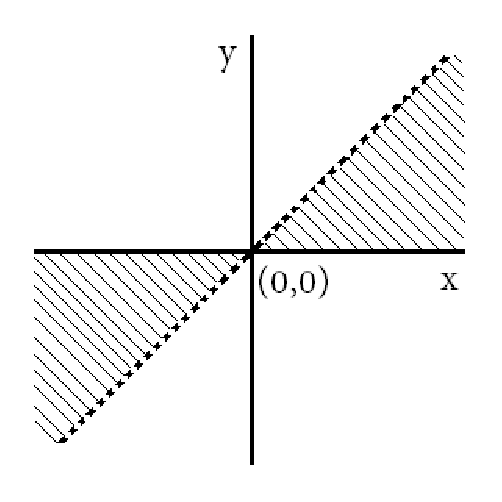
\includegraphics[width=0.8\linewidth]{images/b2p2-278-4a.eps}
	\end{minipage}%
	\\
	\begin{minipage}{0.6\textwidth}\raggedright
		\begin{enumerate}
		\item[b)]\quad $D = {(x, y): x^2 + y - 1 > 0, y \neq 0}$
		\\\noindent
		\quad $D = {(x, y): y > 1 - x^2 , y \neq 0}$
		\end{enumerate}
	\end{minipage}
	\hfill%
	\begin{minipage}{0.3\textwidth}
		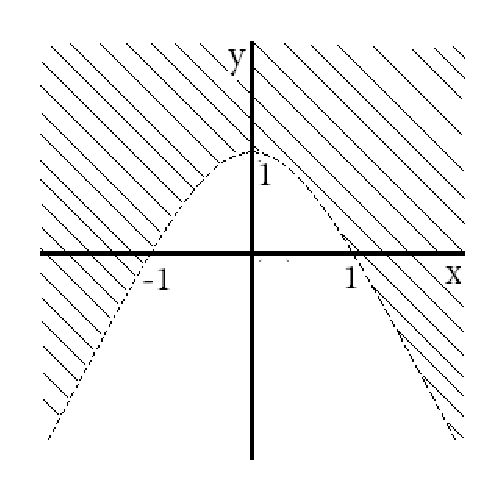
\includegraphics[width=0.8\linewidth]{images/b2p2-278-4b.eps}
	\end{minipage}%
	\\\\
	\noindent
	\item[6.]
	\begin{enumerate}
		\item[a)]\quad $D = {(x, y, z): \frac{|x+y+z-4|}{3} \leqslant 1} = {(x, y, z): 1 \leqslant |x+y+z| \leqslant 1}$
		\\\\\indent\quad
		The region is between and on the parallel planes $x+y+z = 1$, 
		\\\indent\quad $x+y+z = 1$
		\\
		\item[b)]\quad $D = {(x, y, z): z - x^2 - y^2 > 0, y \neq 0}$
		\\\\\indent\quad
		The region is inside the parabaloid $z = x^2 + y^2$ excluding
		\\\indent\quad the plane $y = 0$.	
	\end{enumerate}
	\item[8.]
	\begin{multicols}{2}
	\begin{enumerate}
		\item[a)]\quad 2, \item[b)]\quad 0
	\end{enumerate}
	\end{multicols}	
	\item[10.]
	\begin{multicols}{2}
	\begin{enumerate}
		\item[a)]\quad 1, \item[b)]\quad 1
	\end{enumerate}
	\end{multicols}
	\item[12.]
	\begin{multicols}{2}
	\begin{enumerate}
	\item[a)]\quad independent, \item[b)]\quad dependent
	\end{enumerate}
	\end{multicols}
	\item[14.]
	\begin{multicols}{2}
	\begin{enumerate}
		\item[a)]\quad discontinous \item[b)]\quad discontinous
	\end{enumerate}
	\end{multicols}
	\end{enumerate}
	% =======================================================
\end{document}  